\documentclass[12pt]{article}
%Paquetes a utilizarse
\usepackage[width=7in, height=9.5in, top=0.75in, papersize={8.5in,11in}]{geometry}
\usepackage[spanish]{babel} 
\decimalpoint
\usepackage[utf8]{inputenc}
\usepackage{bbding}
\usepackage[colorlinks = true, linkcolor = blue, urlcolor = BlueViolet, citecolor = OliveGreen]{hyperref}
\usepackage{graphicx}
\usepackage{amssymb,amsthm,amsmath}
\usepackage{enumerate}
\usepackage{array,multicol,multirow}
\usepackage{xcolor}
\usepackage{fancybox,tcolorbox}
\usepackage{caption,subcaption,float,tabularx}
\usepackage{enumitem}

\theoremstyle{definition}
\newtheorem{corolario}{Corolario}
\newtheorem{lema}[corolario]{Lema}
\newtheorem{proposicion}[corolario]{Proposición}
\newtheorem{teorema}[corolario]{Teorema}
\newtheorem{propiedad}[corolario]{Propiedad}
\newtheorem*{observacion}{Observación}
\newtheorem{definicion}{Definición}
\newtheorem*{demostracion}{Demostración}
\newtheorem{ejemplo}{Ejemplo}
\newtheorem{problema}{Problema}
\newtheorem*{solucion}{Solución}
\newtheorem{ejercicio}{\PencilRightDown \  Ejercicio}
\newtheorem{step}{Paso}
\newtheorem{credito}{Crédito}

\usepackage{tikz}
\usetikzlibrary{arrows.meta,babel,calc,positioning}

\renewcommand{\arraystretch}{1.5}
\providecommand{\abs}[1]{\lvert#1\rvert}
\providecommand{\norm}[1]{\lVert#1\rVert}

\renewcommand{\tabularxcolumn}[1]{m{#1}}
\newcommand{\Evaluacion}[4]{
\setcounter{ejercicio}{0}
\noindent\begin{tabular}{lcr}
	\includegraphics[height=3cm]{Logos/logo-UES.png}\hspace{2.5em}
	&
	\includegraphics[height=2.75cm]{Logos/logo-PJT.png}
	& 
	\hspace{2.5em}\includegraphics[height=2.75cm]{Logos/logo-MINEDUCYT.png}
\end{tabular}

\hfill

\begin{center}
    
    UNIVERSIDAD DE EL SALVADOR
    \\PROGRAMA JÓVENES TALENTO
    \\FDTC 2022
    \\#2
    \\Nivel Olímpico C de Matemáticas

\end{center}

\begin{center}
    #1
\end{center}

%\textbf{Nombre}: \enspace\hrulefill

#3

\input{#4}
\newpage
}

\newtheorem{obs}{Observación}

%\usepackage[margin=2.5cm]{geometry}
%\usepackage{wasysym}
%\usepackage{stmaryrd,textcomp}
%\usepackage{pgf,tikz}
%\usetikzlibrary{arrows}

\parskip = 2mm   %%%% genera un espacio de X mm entre lo párrafos
\parindent = 3mm
\usepackage{multicol}
\usepackage{iwona}

\newcommand{\tema}{Introducción}
\newcommand{\fecha}{Lunes, 28 de noviembre de 2022}
\newcommand{\sesion}{Sesión 1}

\begin{document}
%\thispagestyle{empty}
%\newpage
\thispagestyle{empty}

\begin{figure}[h] 
	\begin{minipage}[b]{0.26\textwidth}
		\begin{center}
			
\includegraphics[height=3cm]{Logos/UES.png}
			\par\end{center}
	\end{minipage} 
	\begin{minipage}[b]{0.46\textwidth}
		\begin{center}
			UNIVERSIDAD DE EL SALVADOR\\ [0.1cm]
			PROGRAMA JÓVENES TALENTO\\ [0.1cm]
	        FDTC 2022\\ [0.1cm]
                NIVEL 5\\ [0.1cm]
			COMBINATORIA 
			\par\end{center}
	\end{minipage} 
	\begin{minipage}[b]{0.05\textwidth}
		\begin{center}
			
\includegraphics[height=2cm]{Logos/LOGO PJT.png}
			\par\end{center}
	\end{minipage}
\end{figure}

\begin{center}
    \begin{tabular}{p{4.5cm} p{7cm} p{4.5cm}}
        \tema & \centering\fecha & \hfill\sesion
    \end{tabular}
\end{center}

\section{¿Qué es la combinatoria?}

\subsection{Nociones básicas de la combinatoria}

Cuando alguien se pregunta qué es la combinatoria, una respuesta típica es decir que se trata de ''el arte y la ciencia de contar''. Y es que, al contrario de lo que muchos intuitivamente podrían pensar, contar no es una actividad que siempre resulte ser trivial. En concreto, a la hora de realizar un conteo, nos vamos a enfrentar a dos dificultades elementales: contar todos los elementos y no repetir los elementos contados. Por lo que la combinatoria no solo se trata de ''contar'', sino de ''contar bien''.

Ahora, si bien los métodos de recuento forman parte esencial de la combinatoria, esta también contempla otros aspectos, entre ellos: el estudio de configuraciones conocidas, el estudio de la existencia de ciertas configuraciones, el conteo del número de configuraciones de un tipo dado, la enumeración o descripción de configuraciones, la optimización combinatoria, es decir, la determinación de las configuraciones que maximizan o minimizan una función dada, entre otras. En cualquier caso, el campo abierto a la combinatoria es amplio y fascinante, repleto de bellos resultados e interesantes problemas sin resolver.

En resumen, el conteo es una de las tareas básicas que se realizan en las matemáticas, he aquí su importancia. En este sentido, el objetivo de este curso será ser capaz de determinar cuantos elementos hay, sin caer en la necesidad de contarlos uno a uno.

\subsection{Ejercicios introductorios}

\begin{ejercicio}
    Hay tres caminos que van de la ciudad $A$ a la ciudad $B$, y cuatro caminos que van de la ciudad $B$ a la ciudad $C$. ¿De cuántas maneras podemos ir de la ciudad $A$ a la $C$ pasando por $B$? (No es válido regresarse).
\end{ejercicio}

\begin{ejercicio}
    Hay tres caminos que van de la ciudad $A$ a la ciudad $B$, cuatro caminos que van de la ciudad $B$ a la ciudad $C$, y 5 caminos que van de la ciudad $A$ a la ciudad $C$. ¿De cuántas maneras podemos ir de la ciudad $A$ a la $C$? (No es válido regresarse).
\end{ejercicio}

\begin{ejercicio}
    Disponemos de tres cartas iguales, y de cinco sobres de diferentes colores: amarillo, blanco, café, dorado y escarlata. Vamos a guardar las cartas en los sobres, pero cada sobre puede contener a lo sumo una. ¿De cuántas maneras podemos guardar las cartas en los sobres?
\end{ejercicio}

\begin{ejercicio}
    El garaje de la casa de Ángela tiene cinco plazas. Con ella viven sus hermanas Beatriz y Carmen. Cada una tiene su propio coche, y cada día lo pueden colocar en el lugar queprefieran si no está ocupado. Este es el diagrama de la cochera:

    \begin{center}
        \begin{tabular}{|c|c|c|c|c|}
            1 & 2 & 3 & 4 & 5
        \end{tabular}
    \end{center}

    Por ejemplo, Ángela puede estacionar su coche en el lugar número 1, Beatriz en el número 2, y Carmen en el 4. ¿De cuántas maneras pueden Ángela, Beatriz y Carmen estacionar sus coches?
\end{ejercicio}

\begin{ejercicio}
    Cuatro niños son enviados a un concurso de declamación. Desde luego, todos desean ser el primero en pasar. Supongamos que los niños se llaman Ana, Benito, Carmen y Diego (los llamaremos A, B, C y D). Escriba todos los órdenes posibles en los que podrían pasar a declamar. Por ejemplo, si escribimos A B C D, significa que pasarían en orden Ana, Benito, Carmen y Diego.
\end{ejercicio}

\begin{ejercicio}
    Manuel tiene cuatro carritos de juguete de diferentes colores (azul, blanco, verde y rojo, uno de cada color) y decide regalárselos a sus hermanos Luis y Karen. ¿De cuántas maneras diferentes puede hacer esto? Ejemplo: podría dar los cuatro carritos a Luis. También podría dar tres de ellos a Karen y el otro a Luis.
\end{ejercicio}

\begin{ejercicio}
    En una fiesta, cuatro amigos se van a dar regalos entre sí, de manera que cada uno dé un regalo y reciba otro. Desde luego, nadie debe darse el regalo a sí mismo (algo así como jugar amigo secreto). ¿De cuántas formas es posible hacer la distribución?
\end{ejercicio}

\section{Conjuntos}

\subsection{Nociones básicas de los conjuntos}

\begin{definicion}
    Con el término \textbf{conjunto} nos referimos a ''una colección bien definida de elementos dentro de un todo, considerada en sí misma como un objeto''. El concepto ''bien definido'' significa que para un objeto dado es posible determinar si pertenece o no al conjunto. Los elementos de un conjunto pueden ser casi cualquier cosa: números, personas, letras, etc. Pueden ser incluso otros conjuntos. De forma específica, en matemáticas existen varios conjuntos de números que son especialmente importantes: el conjunto de los números naturales ($\mathbb{N}$), el de los números enteros ($\mathbb{Z}$), el de los números racionales ($\mathbb{Q}$) y el de los números reales ($\mathbb{R}$).
\end{definicion}

Para representar, por ejemplo, que $S$ es el conjunto que contiene los elementos $a, b$ y $c$, escribimos

\begin{center}
    $S=\{a,b,c\}$.
\end{center}

Para indicar que $a$ es un elemento del conjunto $S$, escribimos $a \in S$, y se lee ''$a$ pertenece a $S$''. Generalmente, para nombrar un conjunto, se utilizan letras mayúsculas.

Para definir un conjunto, se puede simplemente elegir o listar cuáles son los elementos que lo componen. También se puede definir un conjunto enunciando una propiedad que permita determinar si un objeto pertenece al conjunto o no. En general, un conjunto puede definirse de dos formas:  por extensión y por comprensión.

\newpage

Por ejemplo, si deseamos expresar que $A$ es el conjunto de los números pares positivos, por extensión tenemos

\begin{center}
    $A=\{2,4,6,8,...\}$
\end{center}

y por comprensión tenemos $A=\{El \ conjunto \ de \ los \ n\Acute{u}meros \ pares \ positivos\}$, o expresado en términos más formales

\begin{center}
    $A=\{2n \ | \ n \in \mathbb{N} \}$
\end{center}

y se lee como ''$A$ es el conjunto de los números de la forma $2n$ tal que $n$ pertenece a los números naturales''. Los símbolos ''$|$'' y ''$:$'' se pueden leer como ''tal que''.

\subsection{Conceptos importantes}

\textbf{Conjunto Vacío:} El conjunto que no tiene  elementos se denomina conjunto vacío, y se representa con el símbolo $\varnothing$, o escribiendo dos llaves: $\{\}$. Cabe resaltar que seconsidera que el conjunto vacío se encuentra incluido en cualquier otro conjunto.

\textbf{Cardinalidad:} A la cantidad de elementos que posee un conjunto se le conoce como la cardinalidad del conjunto, y se denota como $|S|$ donde $S$ es algún conjunto dado. Por ejemplo, si se tiene un conjunto $A=\{a, b, c, d, e\}$ entonces $|A|= 5$. La cardinalidad de un conjunto puede ser infinita, como en el caso de los números naturales, o cero, en el caso del conjunto vacío.

\textbf{Igualdad de Conjuntos:} Dos conjuntos son iguales si y solamente si, poseen los mismos elementos.

\textbf{Subconjuntos:} Si un conjunto $A$ cumple que todos sus elementos también son elementos de otro conjunto $B$, se dice que $A$ es un subconjunto de $B$, o que $A$ está incluido en $B$. Se escribe como $A \subset B$.  Por ejemplo, el conjunto de los números naturales es un subconjunto de los números racionales, es decir, $\mathbb{N} \subset \mathbb{Q}$. Además, todo conjunto es subconjunto de sí mismo.

\textbf{Conjunto Potencia:} Dado un conjunto $A$, se le denomina conjunto potencia de $A$, al conjunto cuyos elementos son todos los subconjuntos de $A$ y se denota por $P(A)$. Por ejemplo, si $A=\{a,b\}$, entonces $P(A)=\{\varnothing,\{a\},\{b\},\{a,b\}\}$.

\subsection{Operaciones con conjuntos}

Típicamente, se utilizan diagramas de Venn para visualizar el comportamiento de los conjuntos gráficamente.

\begin{center}
    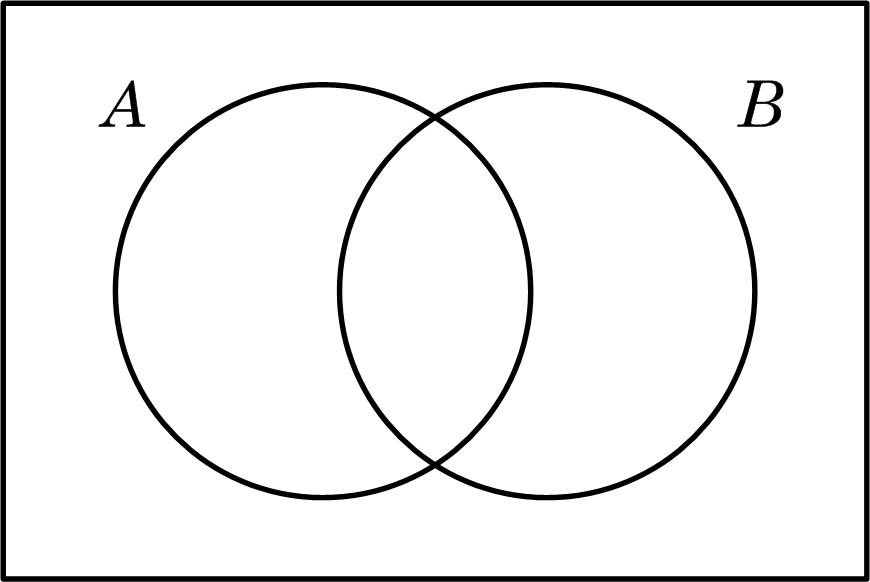
\includegraphics[height=3cm]{Imagenes/IMG1/Venn.png}
\end{center}

\textbf{Unión de conjuntos:} Sean $A$ y $B$ dos conjuntos. Entonces, el conjunto unión de $A$ con $B$ se denota por $A \cup B$, y está formado por todos los elementos que pertenecen al conjunto $A$, al conjunto $B$, o a ambos.

\begin{center}
    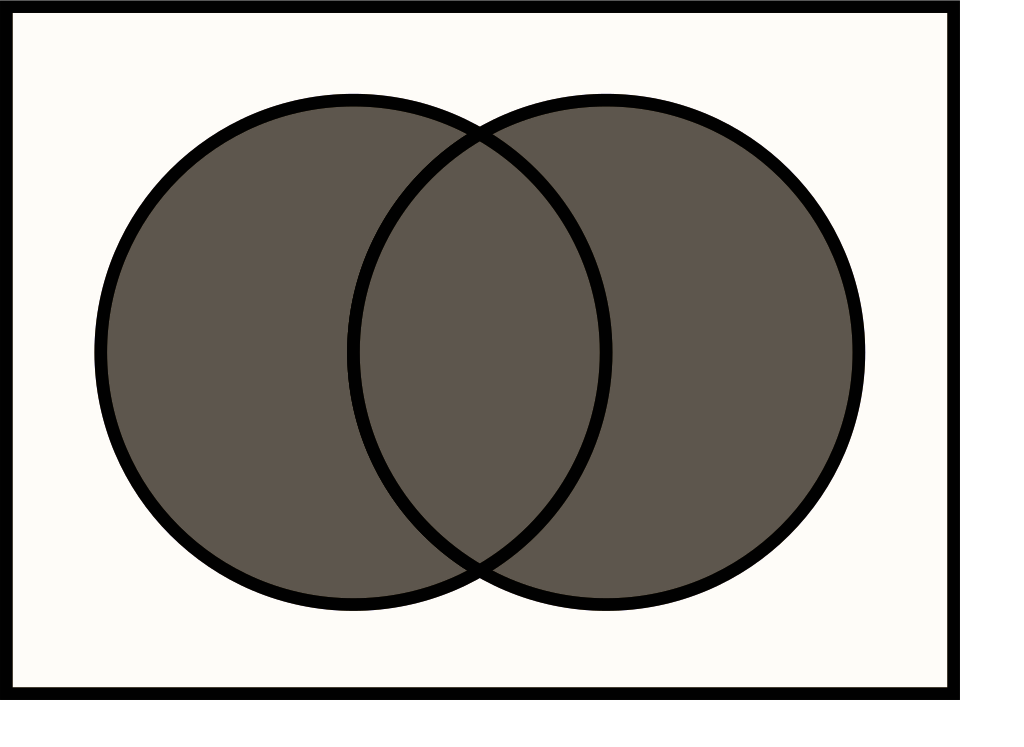
\includegraphics[height=3cm]{Imagenes/IMG1/Union.png}
\end{center}

\begin{ejemplo}
    Sea $A=\{x \ | \ x \in \mathbb{N}, \ 10 \leq x < 14\}$ y $B=\{y \ | \ y \ es \ par, \ 6<y<18\}$. Encontrar $A \cup B$.
\end{ejemplo}

\begin{solucion}
    Se deben definir los conjuntos por extensión, por lo que $A=\{10,11,12,13\}$ y $B=\{8,10,12,14,16\}$.  Entonces, $A \cup B=\{8,10,11,12,13,14,16\}$.
\end{solucion}

\textbf{Intersección de conjuntos:} Sean $A$ y $B$ dos conjuntos. Entonces, el conjunto intersección de $A$ y $B$ se denota por $A \cap B$, y está formado solo por los elementos que pertenecen a ambos conjuntos.

\begin{center}
    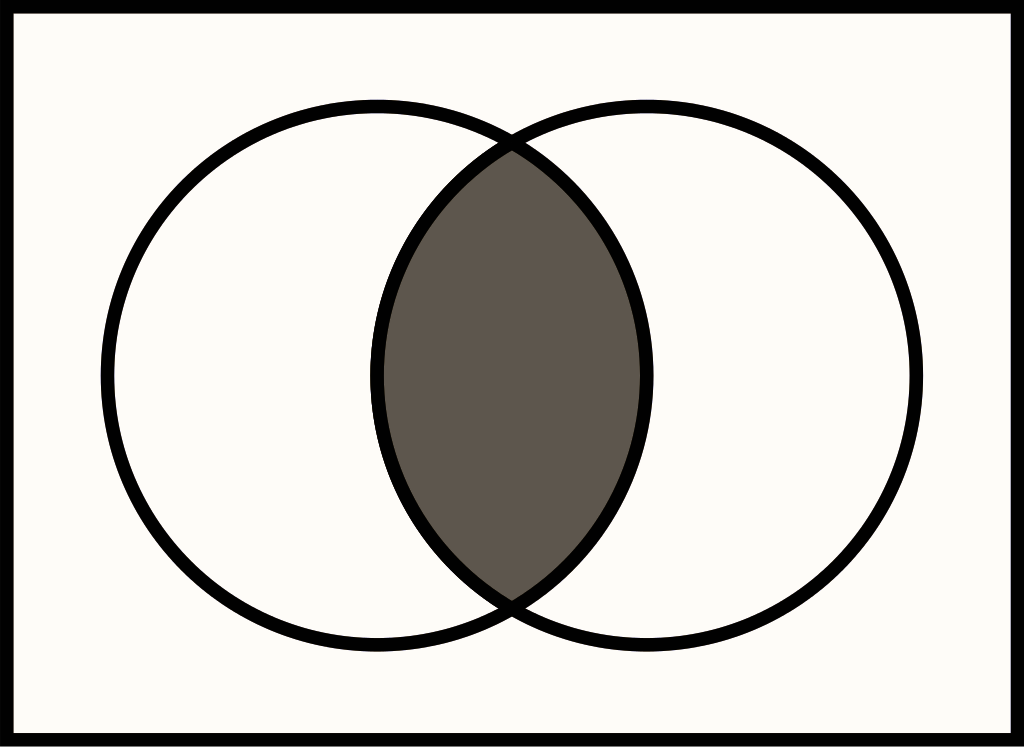
\includegraphics[height=3cm]{Imagenes/IMG1/Interseccion.png}
\end{center}

\begin{ejemplo}
    Si $A=\{las \ vocales\}$ y $B=\{x \ | \ x \ es \ una \ letra \ de \ la \ palabra \ COMBINATORIA\}$, hallar $A \cap B$.
\end{ejemplo}

\begin{solucion}
    Al definir los conjuntos por extensión, tenemos que $A=\{a,e,i,o,u\}$ y, eliminando las repreticiones, $B=\{c,o,m,b,i,n,a,t,r\}$.  Por lo tanto, los elementos en común son $A \cap B=\{a,i,o\}$.
\end{solucion}

\textbf{Diferencia de conjuntos:} Sean $A$ y $B$ dos conjuntos. Entonces, se denota por $A-B$ al conjunto formado por todos los elementos de $A$ que no pertenecen a $B$. De cierta forma significa ''quitarle a $A$ todos los elementos que también pertenecen a $B$''.

\begin{center}
    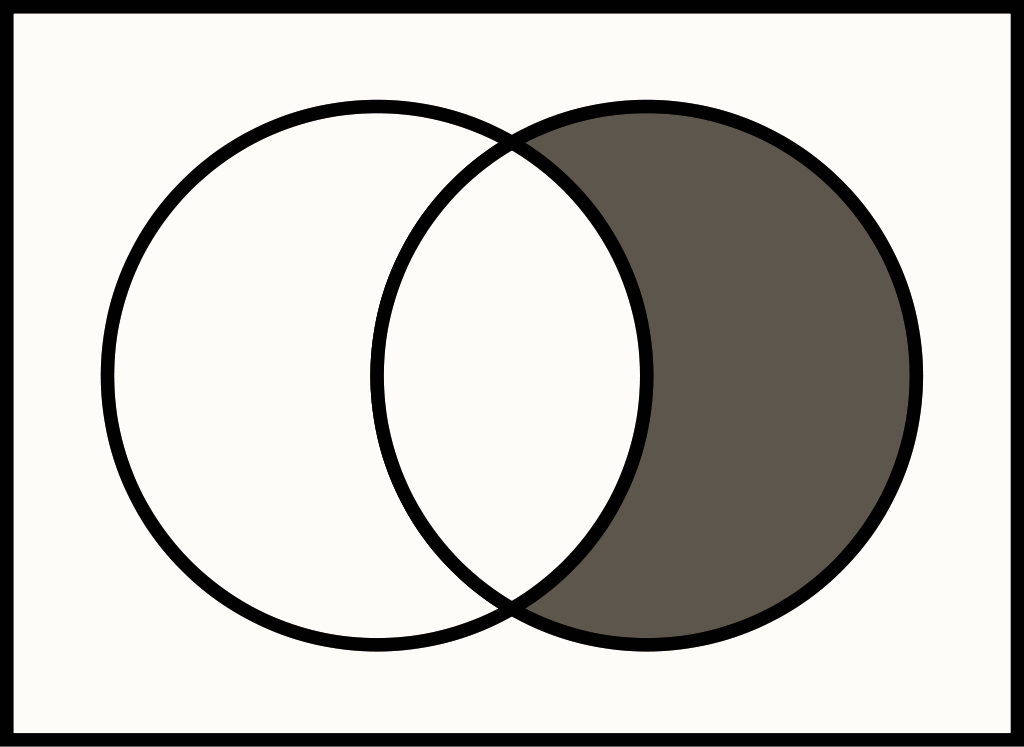
\includegraphics[height=3cm]{Imagenes/IMG1/Diferencia.png}
\end{center}

\begin{ejemplo}
    Si se tiene que $A=\{-5,1,-3,2,-2,9\}$ y $B=\{x \ | \ x \in \mathbb{N} \}$, ¿cuáles son los elementos de $A-B$?
\end{ejemplo}

\begin{solucion}
    El conjunto $A$ ya esta difinido por extensión y $B$ es el conjunto de los números naturales.  Al quitarle a $A$ todos los elementos que también pertenecen a $B$, nos resulta $A-B=\{-5,-3,-2\}$.
\end{solucion}

\textbf{Complemento de un conjunto:} Sea $A$ un subconjunto de cierto conjunto $U$. Entonces el conjunto complemento de $A$ dentro del conjunto $U$, se denota por $A^C$ o por $A'$, y está compuesto por todos los elementos de $U$ que no pertenecen a $A$.

\begin{center}
    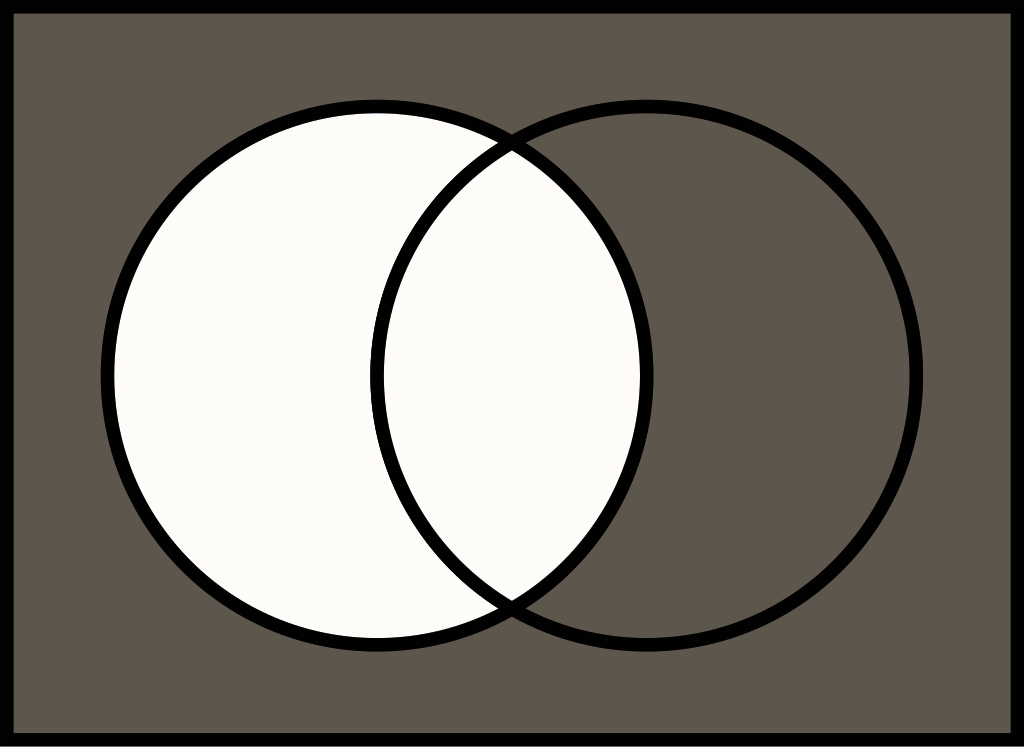
\includegraphics[height=3cm]{Imagenes/IMG1/Complemento.png}
\end{center}

\begin{ejemplo}
    Si $A$ es el conjunto de los números enteros positivos ($\mathbb{Z}^{+}$) y $U$ son los números enteros ($\mathbb{Z}$). ¿Quién es $A^C$?
\end{ejemplo}

\begin{solucion}
    Bajo la idea de complemento se puede hacer la iguiente pregunta:  ¿qué le hace falta a $\mathbb{Z}^{+}$ para ser el conjunto de los $\mathbb{Z}$?.  Al responder la pregunta, nos damos cuenta de que $A^C=\mathbb{Z}^{-}_{0}$.
\end{solucion}

\begin{ejemplo}
    Si se tienen los conjuntos:

    \begin{center}
        $A =\{0, 1, 2, 7, 8\}$ \\
        $B =\{1, 3, 4, 5, 8\}$ \\
        $U =\{0, 1, 2, 3, 4, 5, 6, 7, 8, 9\}$
    \end{center}

    Determinar $A \cup B$, $A \cap B$, $A-B$ y $A^C$. Además, determinar $|A|$, $|B|$, $|A \cap B|$ y $|A \cup B|$. ¿Nota alguna relación entre estas cardinalidades?
    
\end{ejemplo}

\begin{solucion} Los resultados de las operaciones serían

    \begin{center}
        $A \cup B=\{0,1,2,3,4,5,7,8\}$ \\
        $A \cap B=\{1,8\}$ \\
        $A-B=\{0,2,7\}$ \\
        $A^C=\{3,4,5,6,9\}$ \\
        $|A|=5$, $|B|=5$, $|A \cap B|=2$ y $|A \cup B|=8$
    \end{center}

    Notar que, para cualesquiera par de conjuntos, se cumple que $|A \cup B| = |A| + |B| - |A \cap B|$.
    
\end{solucion}

\subsection{Problemas}

\begin{problema}
    Encuentre la intersección de
    \renewcommand{\labelenumi}{\alph{enumi})}
    \begin{enumerate}
        \item $\{3,4,5,6,7\}$ y $\{4,6,8,10\}$
        \item $\{9,14,25,30\}$ y $\{10,17,19,38,52\}$
    \end{enumerate}
\end{problema}

\begin{problema}
    Encuentre la unión de
    \renewcommand{\labelenumi}{\alph{enumi})}
    \begin{enumerate}
        \item $\{a,b,d,f,g,h\}$ y $\{c,f,g,h,k\}$
        \item $\{3,4,5\}$ y $\varnothing$
    \end{enumerate}
\end{problema}

\newpage

\begin{problema}
    Sea $U=\{1,2,3,4,5,6,9\}$, $A=\{1,2,3,4\}$, $B=\{2,4,6\}$ y $C=\{3,5,7\}$. Encuentre y grafique en diagramas de Venn:
    \renewcommand{\labelenumi}{\alph{enumi})}
    \begin{enumerate}
        \item $A' \cap B$
        \item $B' \cup C'$
        \item $A \cap (B \cup C')$
        \item $(A' \cup C') \cap (B')$
    \end{enumerate}
\end{problema}

\begin{problema}
    Sea $U=\{1,2,3,4,5,6,7\}$, $A=\{1,2,3,4,5,6\}$, $B=\{2,3,6\}$ y $C=\{3,5,7\}$. Encuentre:
    \renewcommand{\labelenumi}{\alph{enumi})}
    \begin{enumerate}
        \item $A-B$
        \item $B-A$
        \item $(A-B) \cup C)$
    \end{enumerate}
\end{problema}

\begin{problema}
    Suponga que se tienen dos conjuntos $A$ y $B$. Sombree en un diagrama de Venn las regiones que hacen referencia a las siguientes operaciones:
    \renewcommand{\labelenumi}{\alph{enumi})}
    \begin{enumerate}
        \item $(A \cap B)'$
        \item $A' \cup B'$
        \item $(A \cup B)'$
        \item $A' \cap B'$
    \end{enumerate}
    A estas propiedades se les conoce como \textbf{leyes de De Morgan}.
\end{problema}

\end{document}